\section{Alex Pitcher Report - Part III}

\subsection{Happy birthday Zdenko}

Myself and Dave exited the cave the day before there was to be a
birthday party held for the current head of the JSPDT, Z\sidenote{Zdenko Rejec}. The next day,
we deserted the plateau and made headway for the Shepherds Huts further
down the mountain. Here, we were greeted warmly by a glass of jaganje,
as is and served up some delicious Slovenian food. One of my favourite
memories of Slovenia will be watching the sun set over \passage[town]{Tolmin} that night
as \bignote{I finally felt at home on the expedition and with caving}. As the
night continued, the night became more hazy as we all drank a large
amount of red wine and watched what was a crazy yet hilarious birthday
ceremony involving someone dressed up blessing Z. The wine eventually
took its toll and somehow I found my way to sleep.

\begin{pagefigure}
      \checkoddpage \ifoddpage \forcerectofloat \else \forceversofloat \fi
    \centering
    \begin{subfigure}{0.49\textwidth}
        \frame{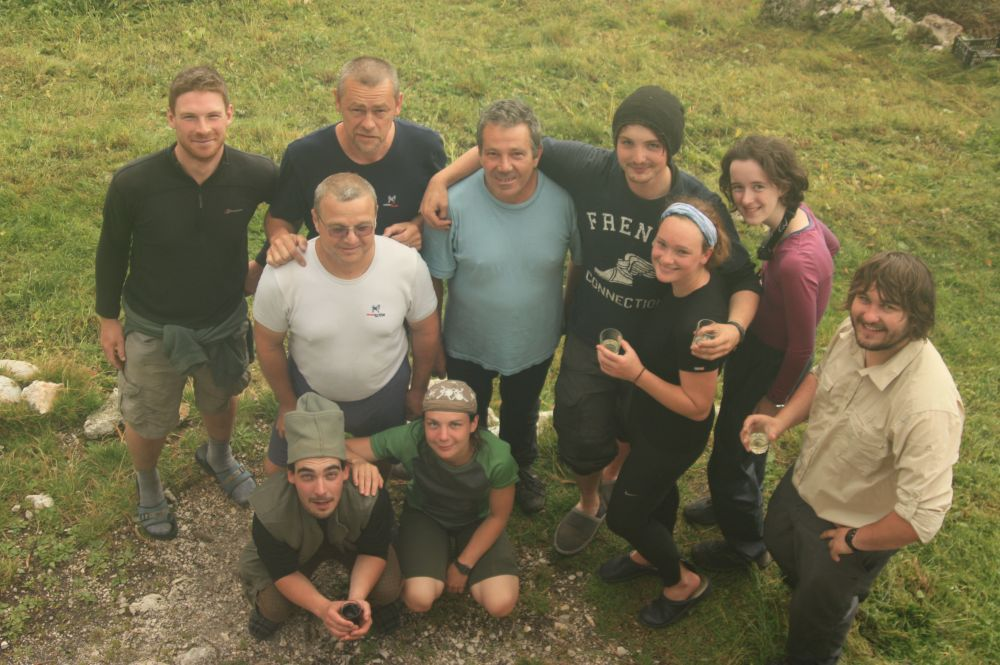
\includegraphics[width=\linewidth]{2011/alex_pitcher_award/zdenko/2011-08-06-16.48.07-Gergely Ambrus-Canon450D-IMG_1030-Zdenkos 50th Birthday Party at Kal--orig.jpg}}
        \caption{}
    \end{subfigure}
\hfill
    \begin{subfigure}{0.49\textwidth}
    \centering
        \frame{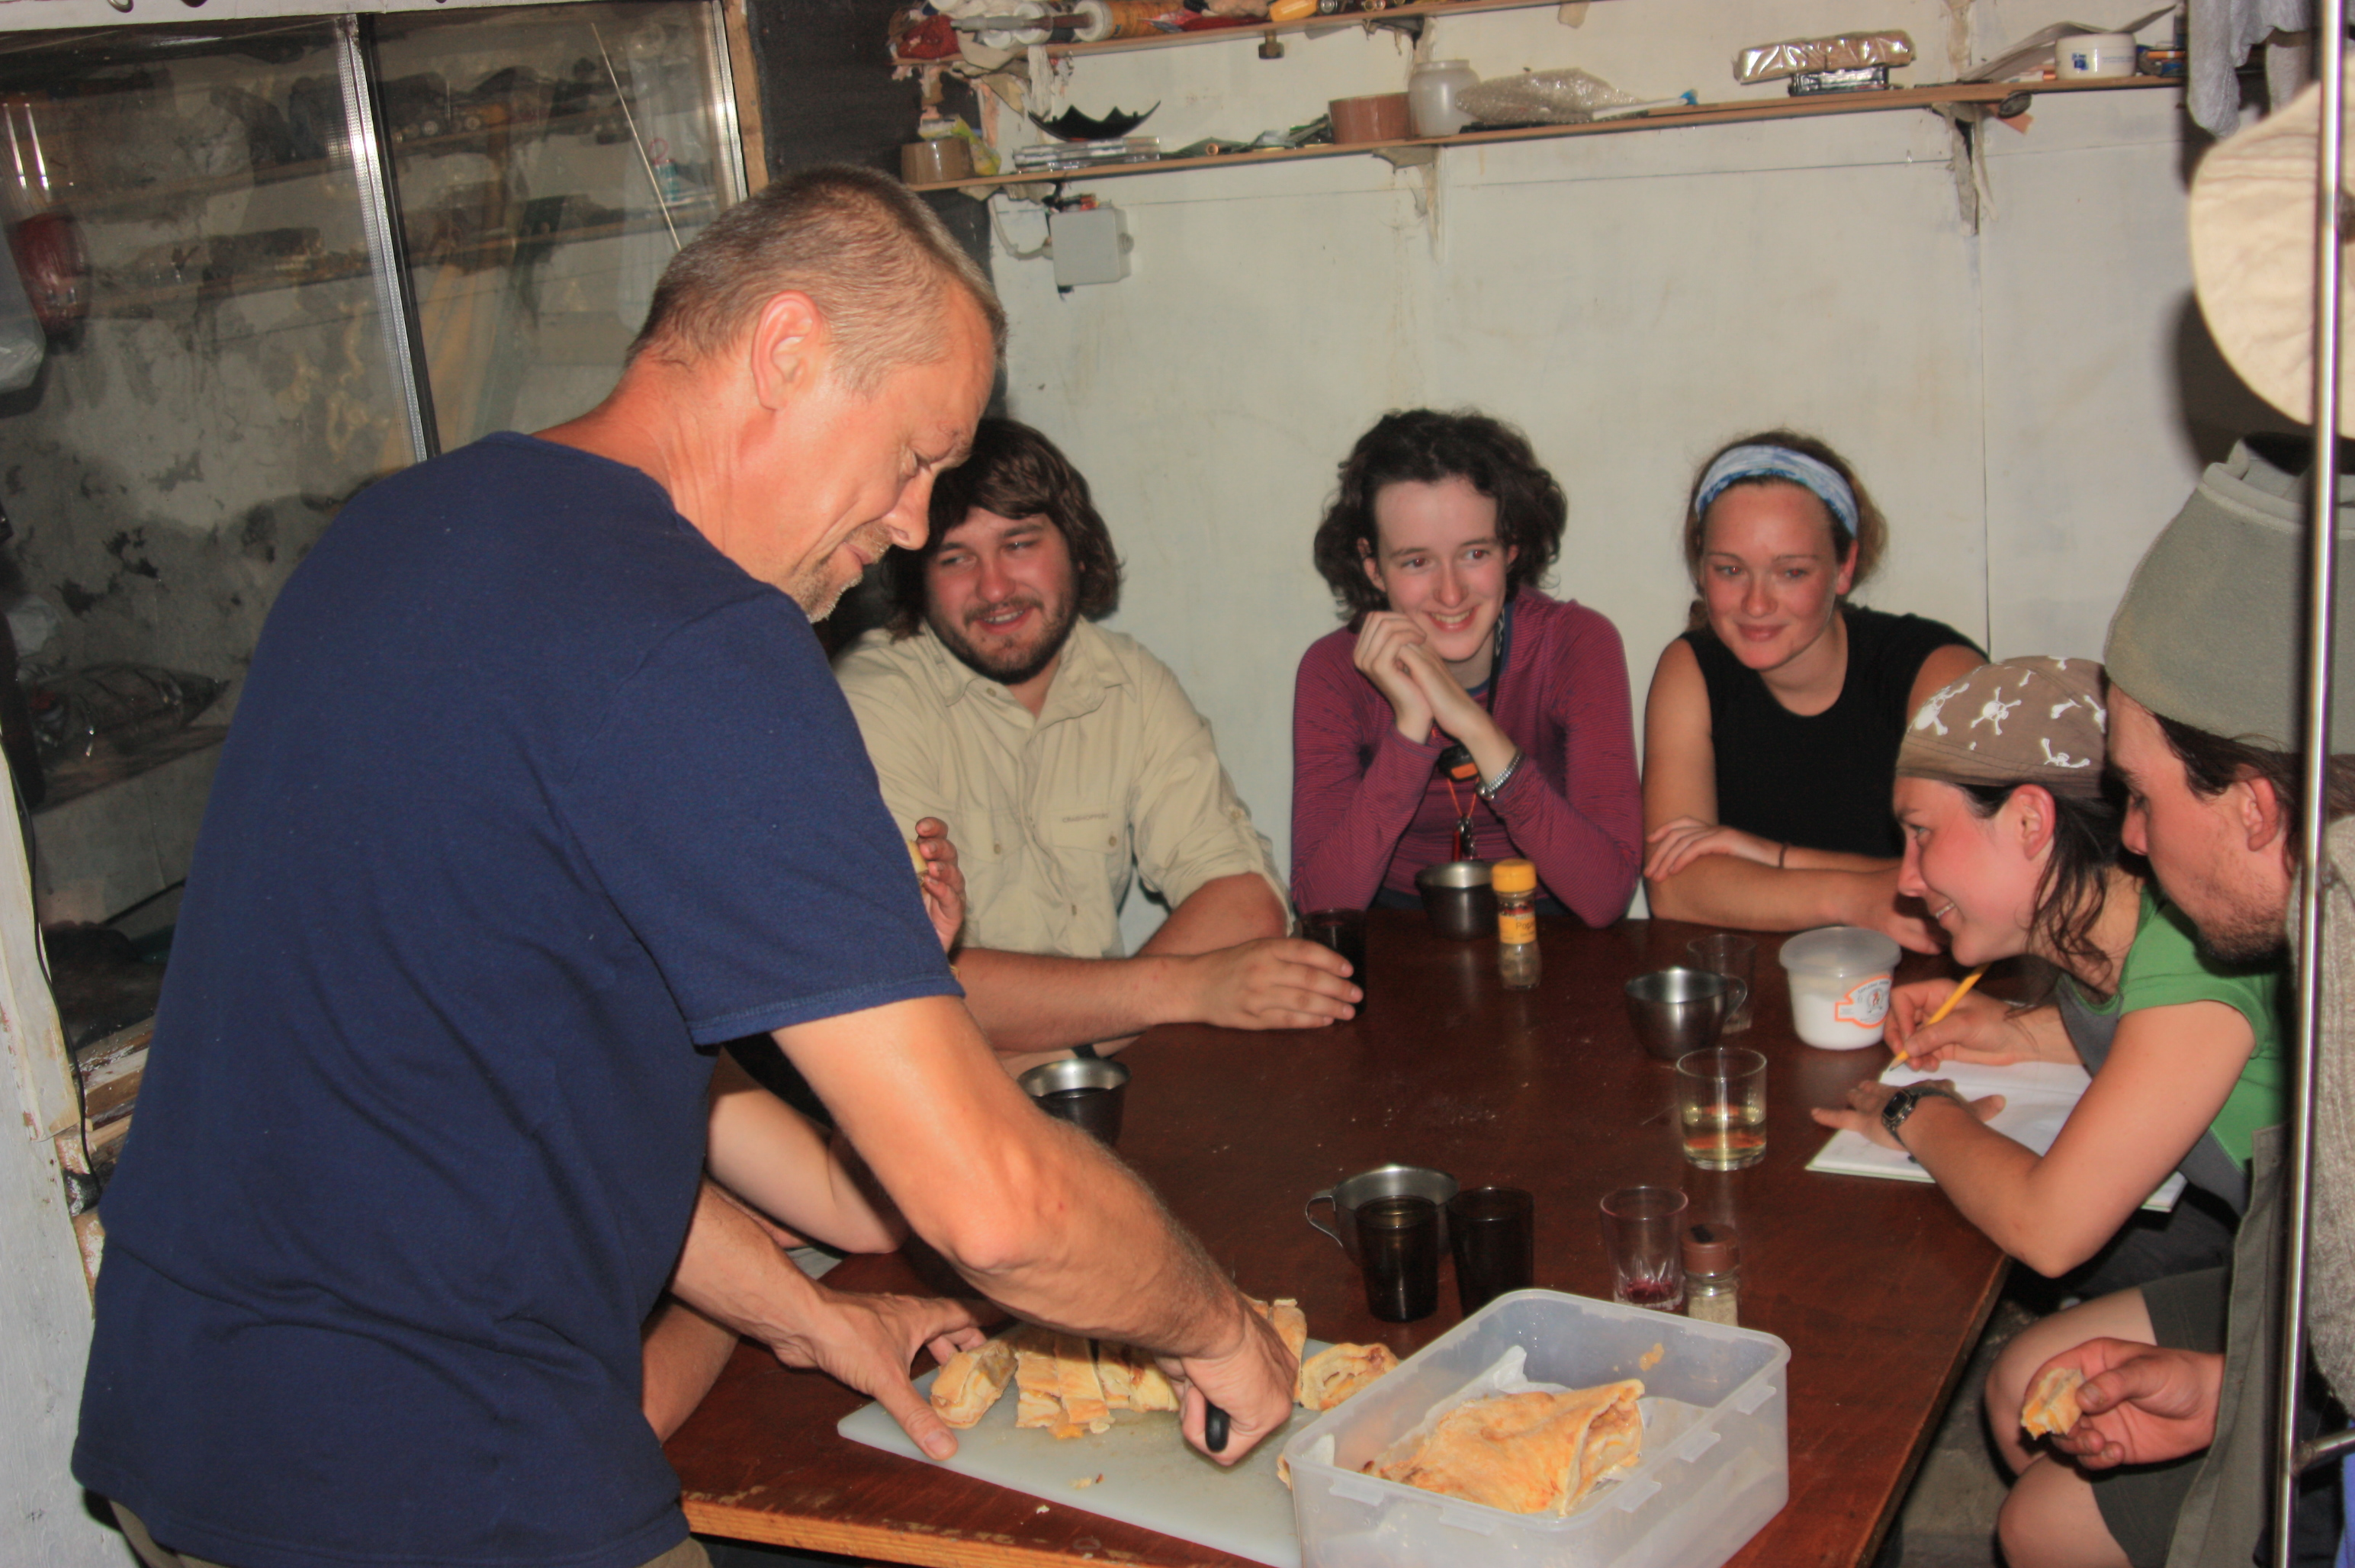
\includegraphics[width=\linewidth]{2011/alex_pitcher_award/zdenko/2011-08-06-17.15.16-Gergely Ambrus-Canon450D-IMG_1033-Zdenkos 50th Birthday Party at Kal--orig.jpg}}
        \caption{}
\end{subfigure}
\vfill
\begin{subfigure}{0.49\textwidth}
    \centering
        \frame{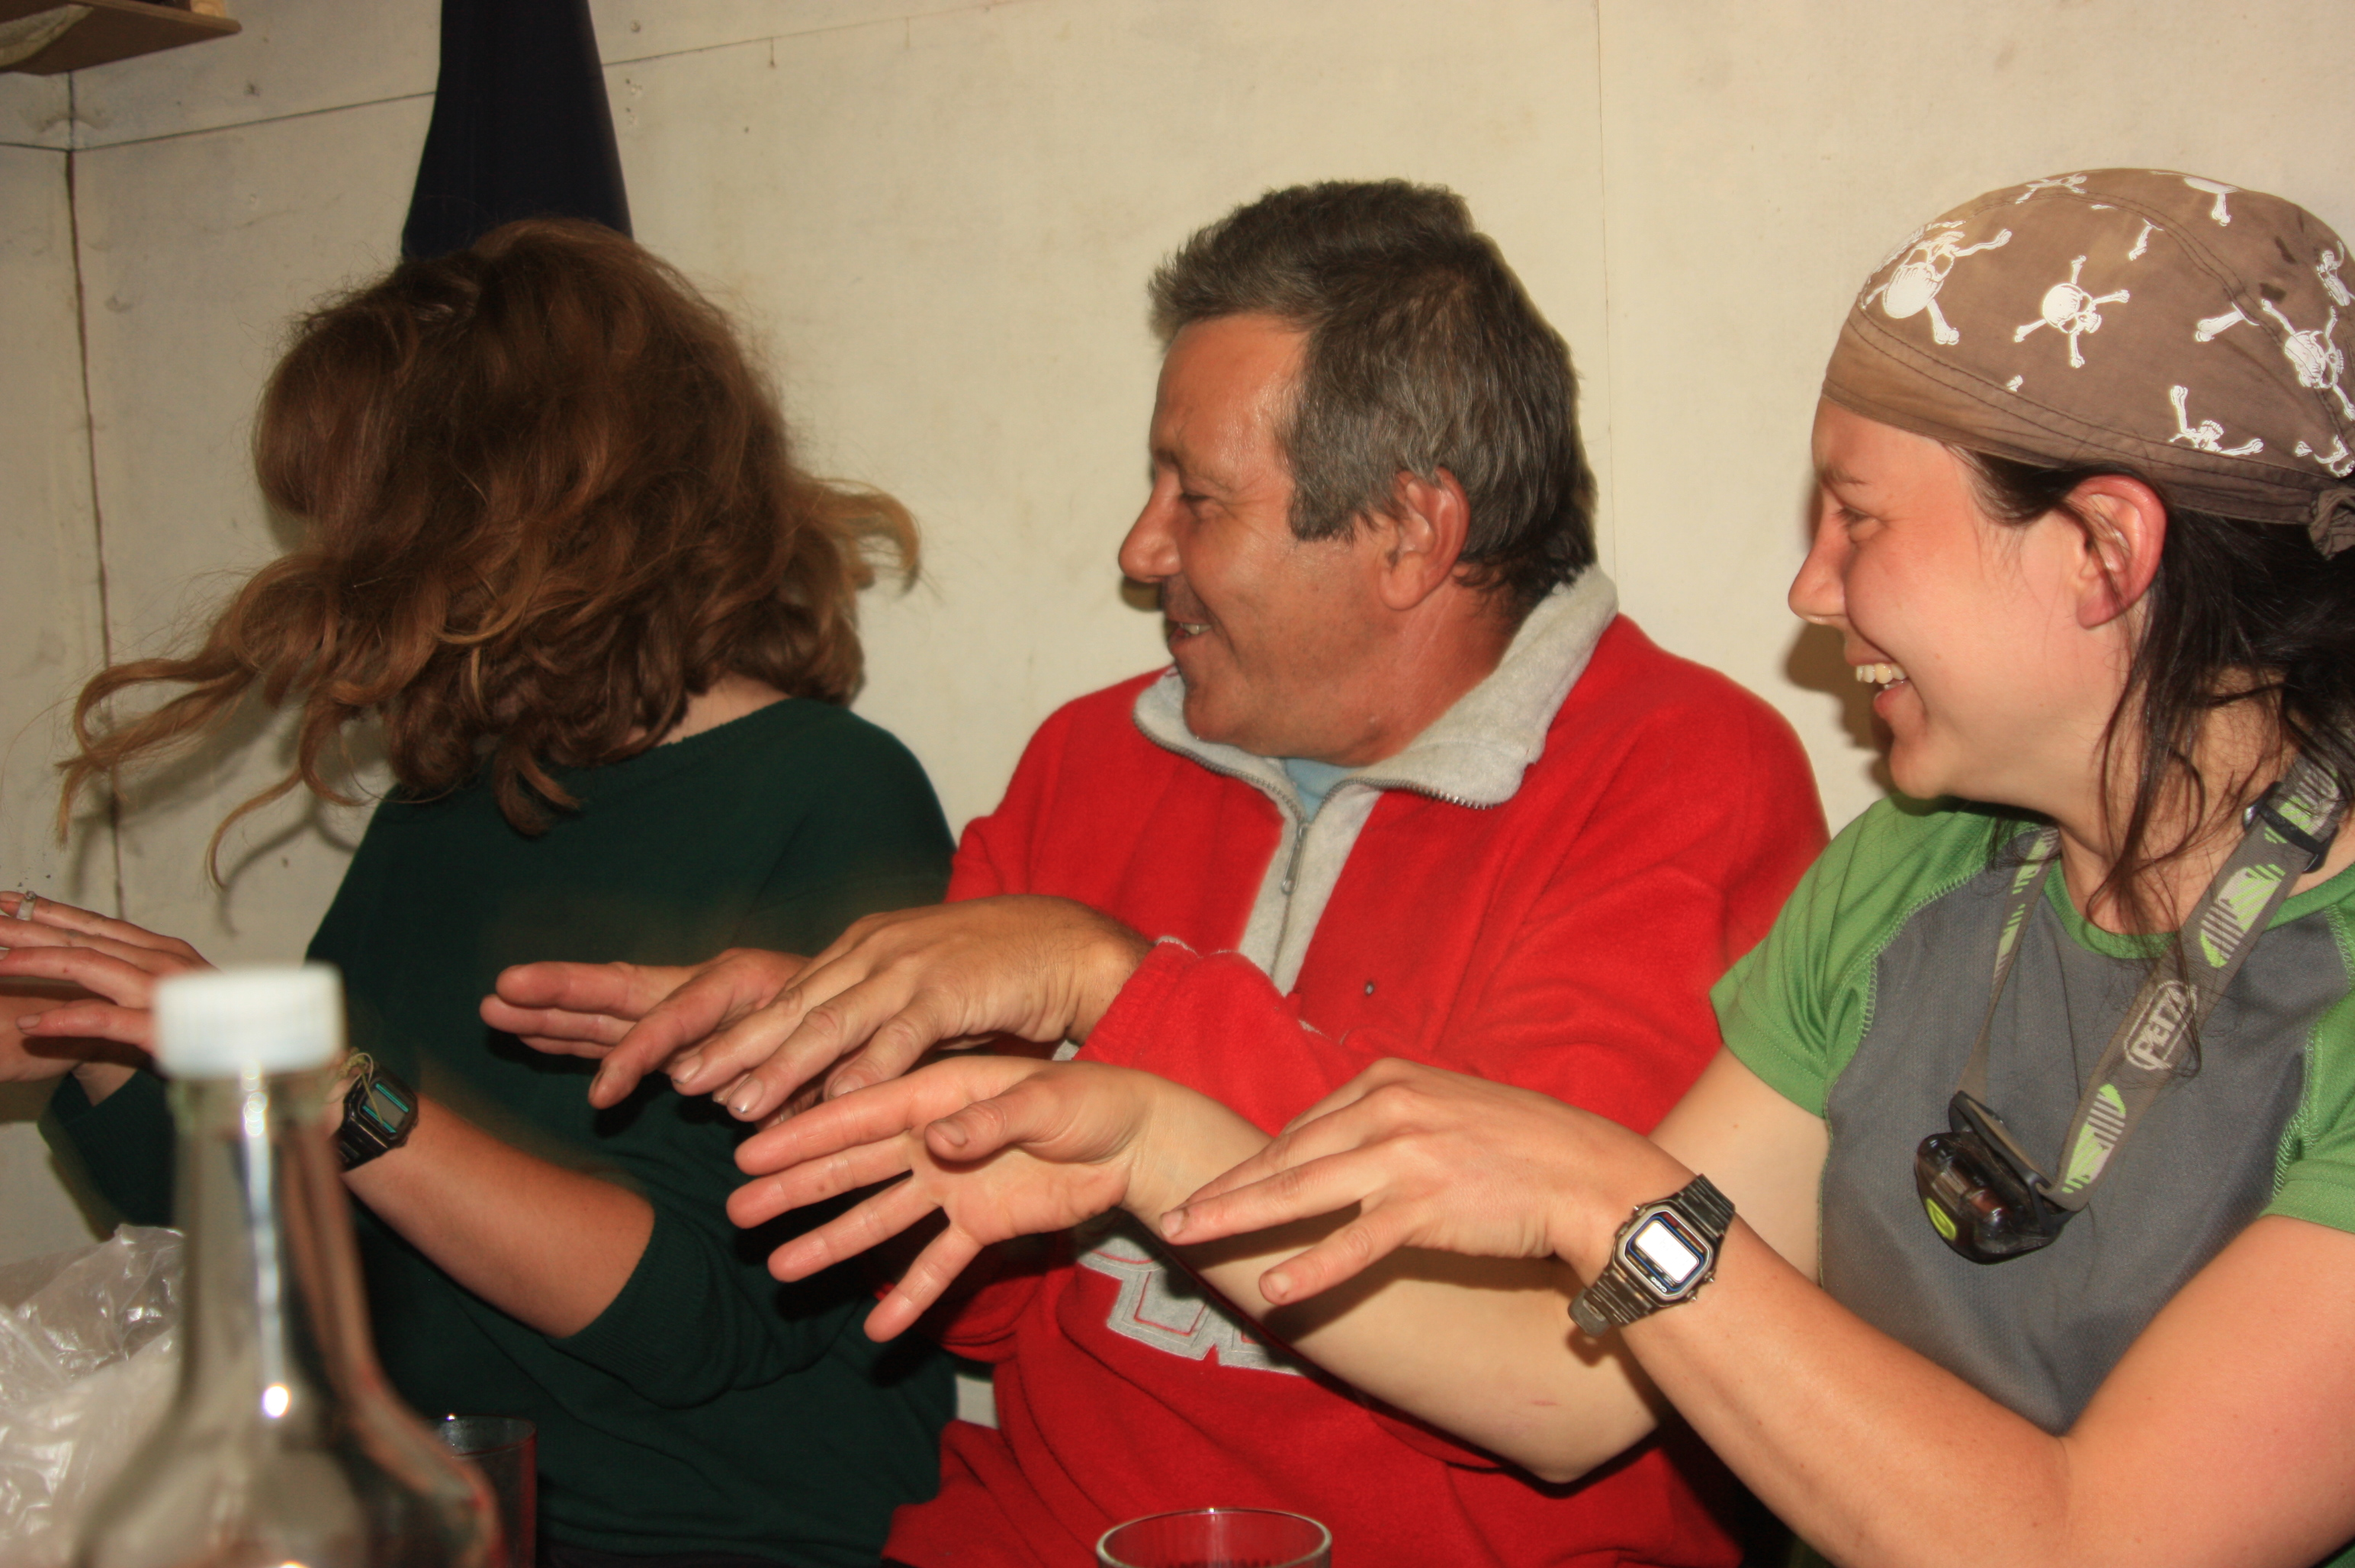
\includegraphics[width=\linewidth]{2011/alex_pitcher_award/zdenko/2011-08-06-22.39.02-Gergely Ambrus-Canon450D-IMG_1117-Zdenkos 50th Birthday Party at Kal--orig.jpg}}
        \caption{}
\end{subfigure}
\hfill
\begin{subfigure}{0.49\textwidth}
    \centering
        \frame{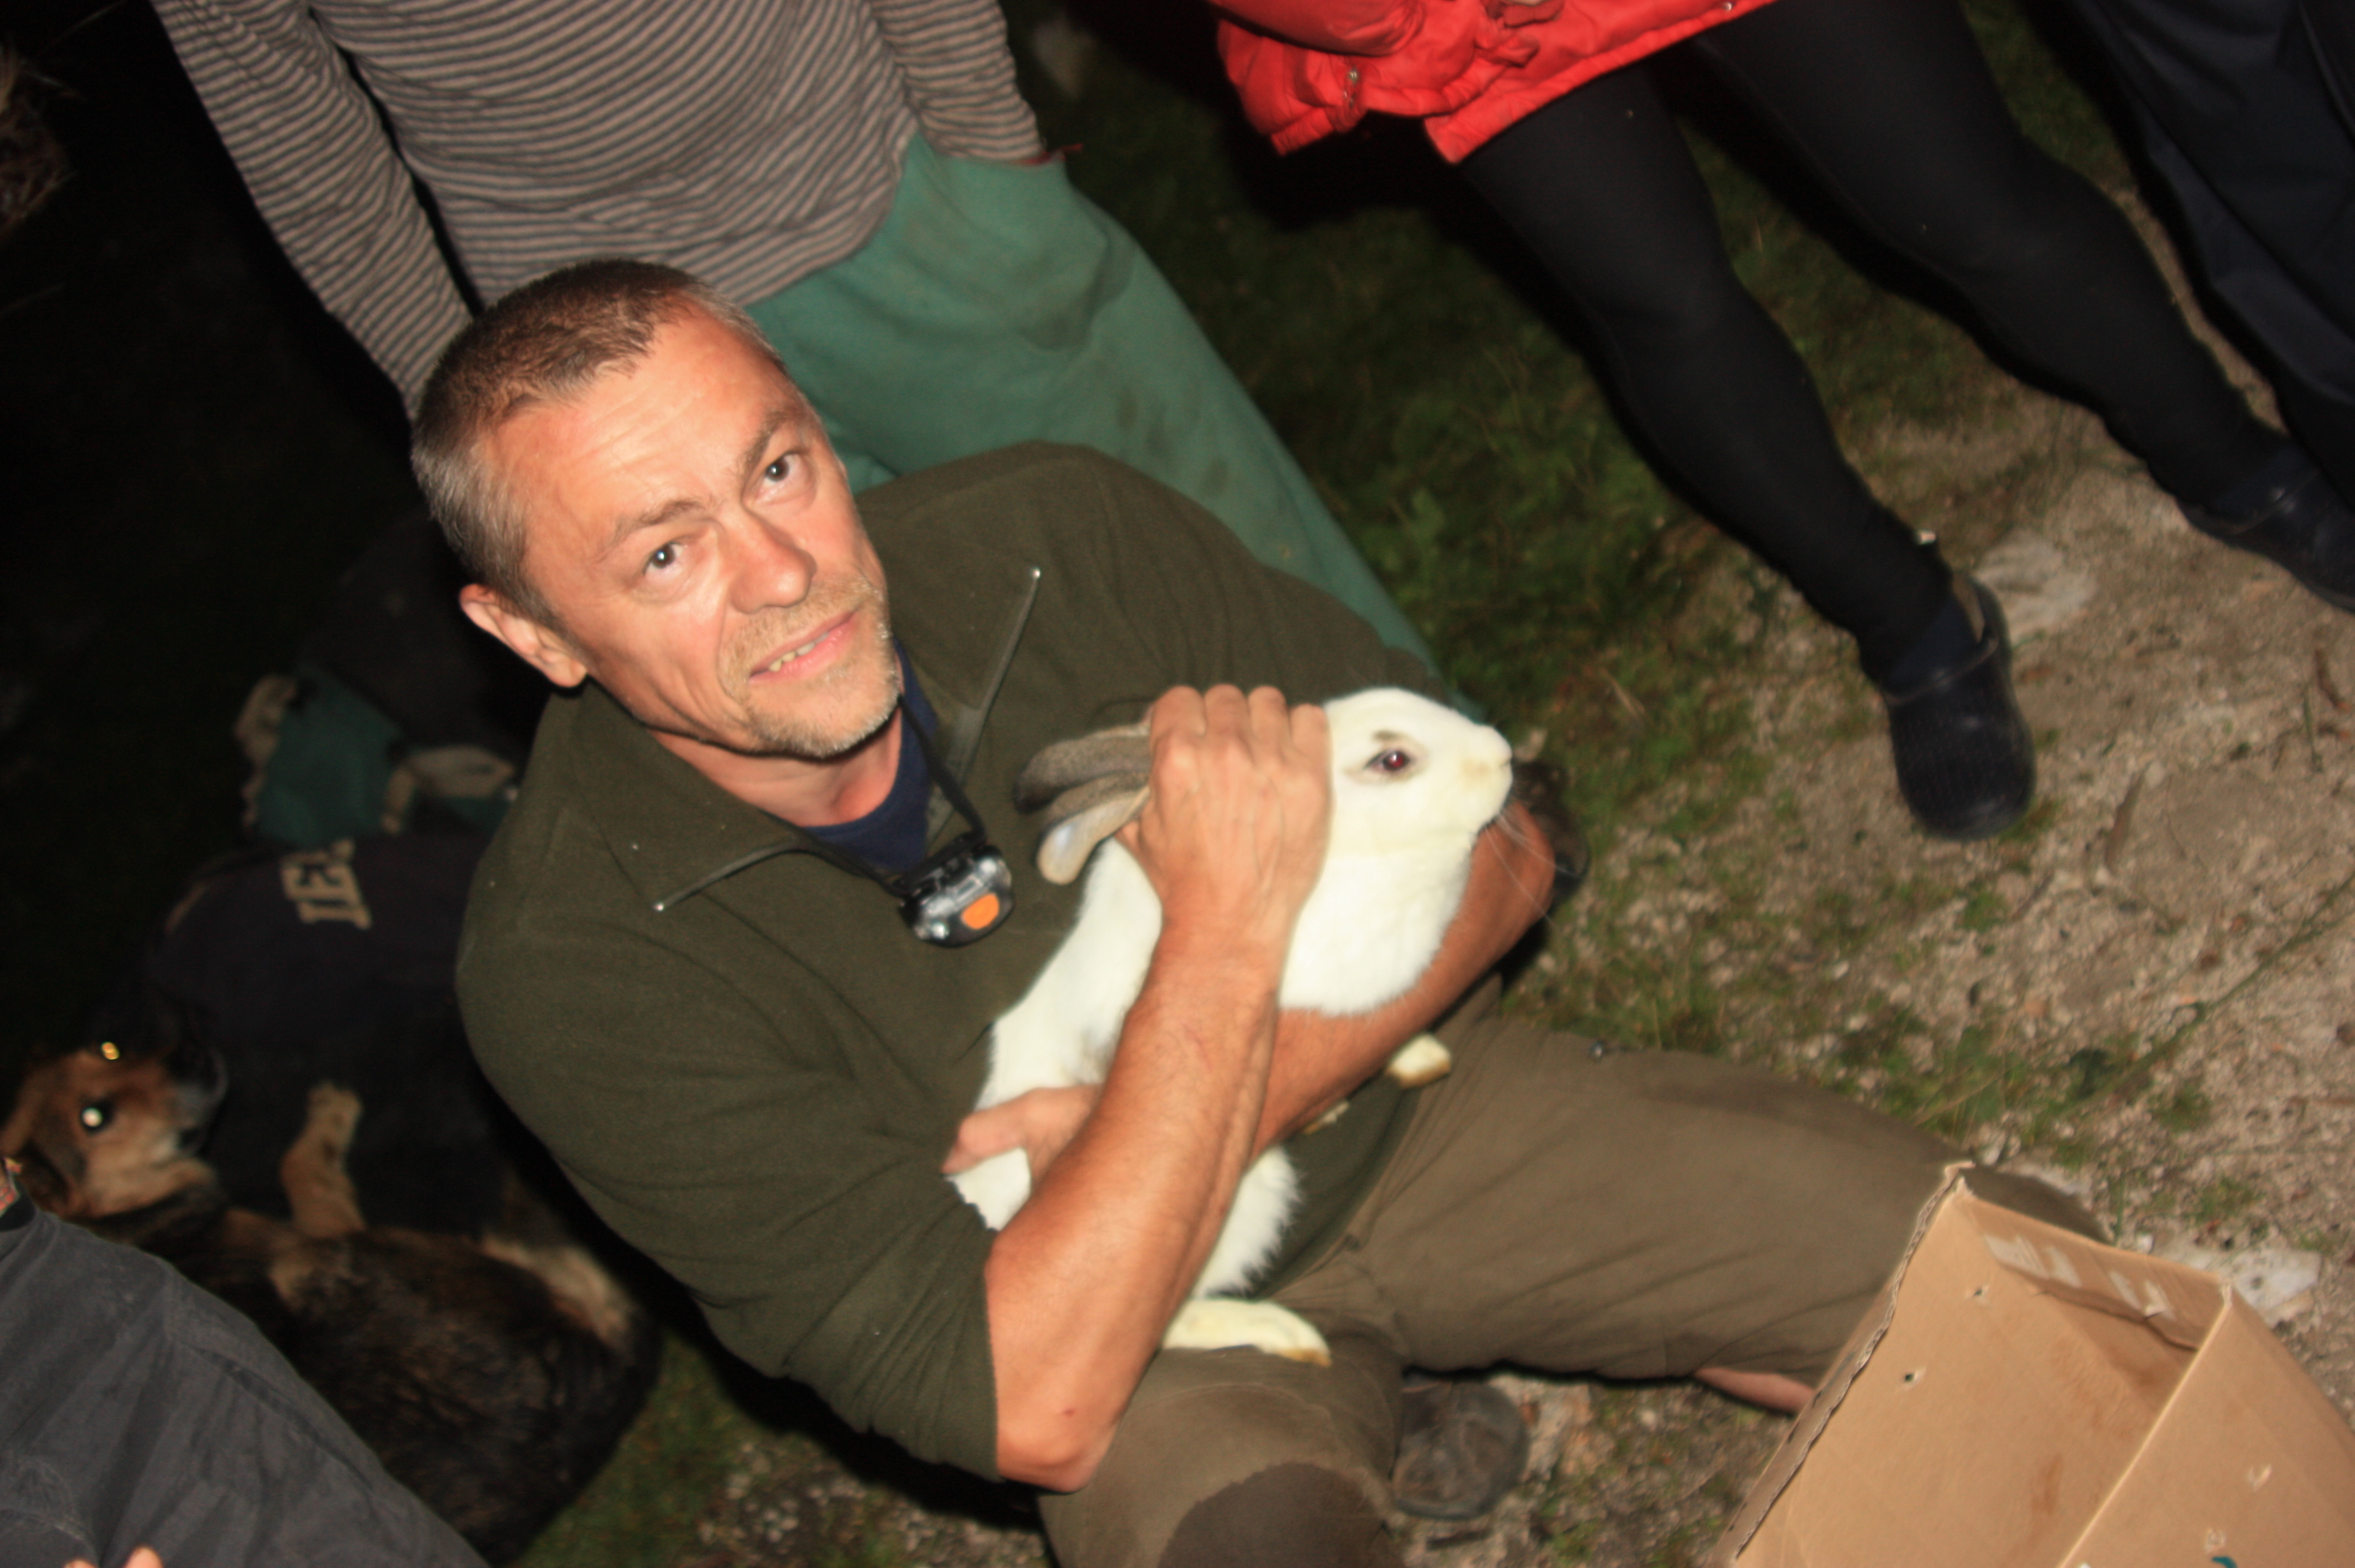
\includegraphics[width=\linewidth]{2011/alex_pitcher_award/zdenko/2011-08-06-23.50.57-Gergely Ambrus-Canon450D-IMG_1195-Zdenkos 50th Birthday Party at Kal--orig.jpg}}
        \caption{}
    \end{subfigure}
\caption{Zdenko's 50th birthday party at \passage{Planina Kal}. It can be assumed that the evening passed in a blur of merry festivities that don't need individual descriptions. \pic{Gergely Ambrus}}
\end{pagefigure}


\subsection{Derigging \passage{Vrtnarija}}

The following morning, I awoke feeling worse for wear missing one of my
trouser legs (I still don't know what happened to it) and made plans to
head back to the plateau. It was the final week and the expedition was
finally coming to an end. Thoughts were turning to the mammoth derig
that awaited us in the cave. Throughout the year just over 2 km of cave had
been found by the ICCC and JSPDT and I'm sure everyone on the mountain
felt immensely proud. The cave was now at a depth of 888 m and a length
of 11025 m. Now, however, camp had to be packed up and brought back to
the surface whilst the rope from the pitches down to camp had to be
taken down and all the hangers and maillons removed and brought to the
surface. All the cavers available and able to help were to embark on a
bounce trip down to camp to collect at least a tackle bag each.
Throughout the day we all set off at different times for what was to be
the last trip of the year.

\begin{marginfigure}
\checkoddpage \ifoddpage \forcerectofloat \else \forceversofloat \fi
\centering
 \frame{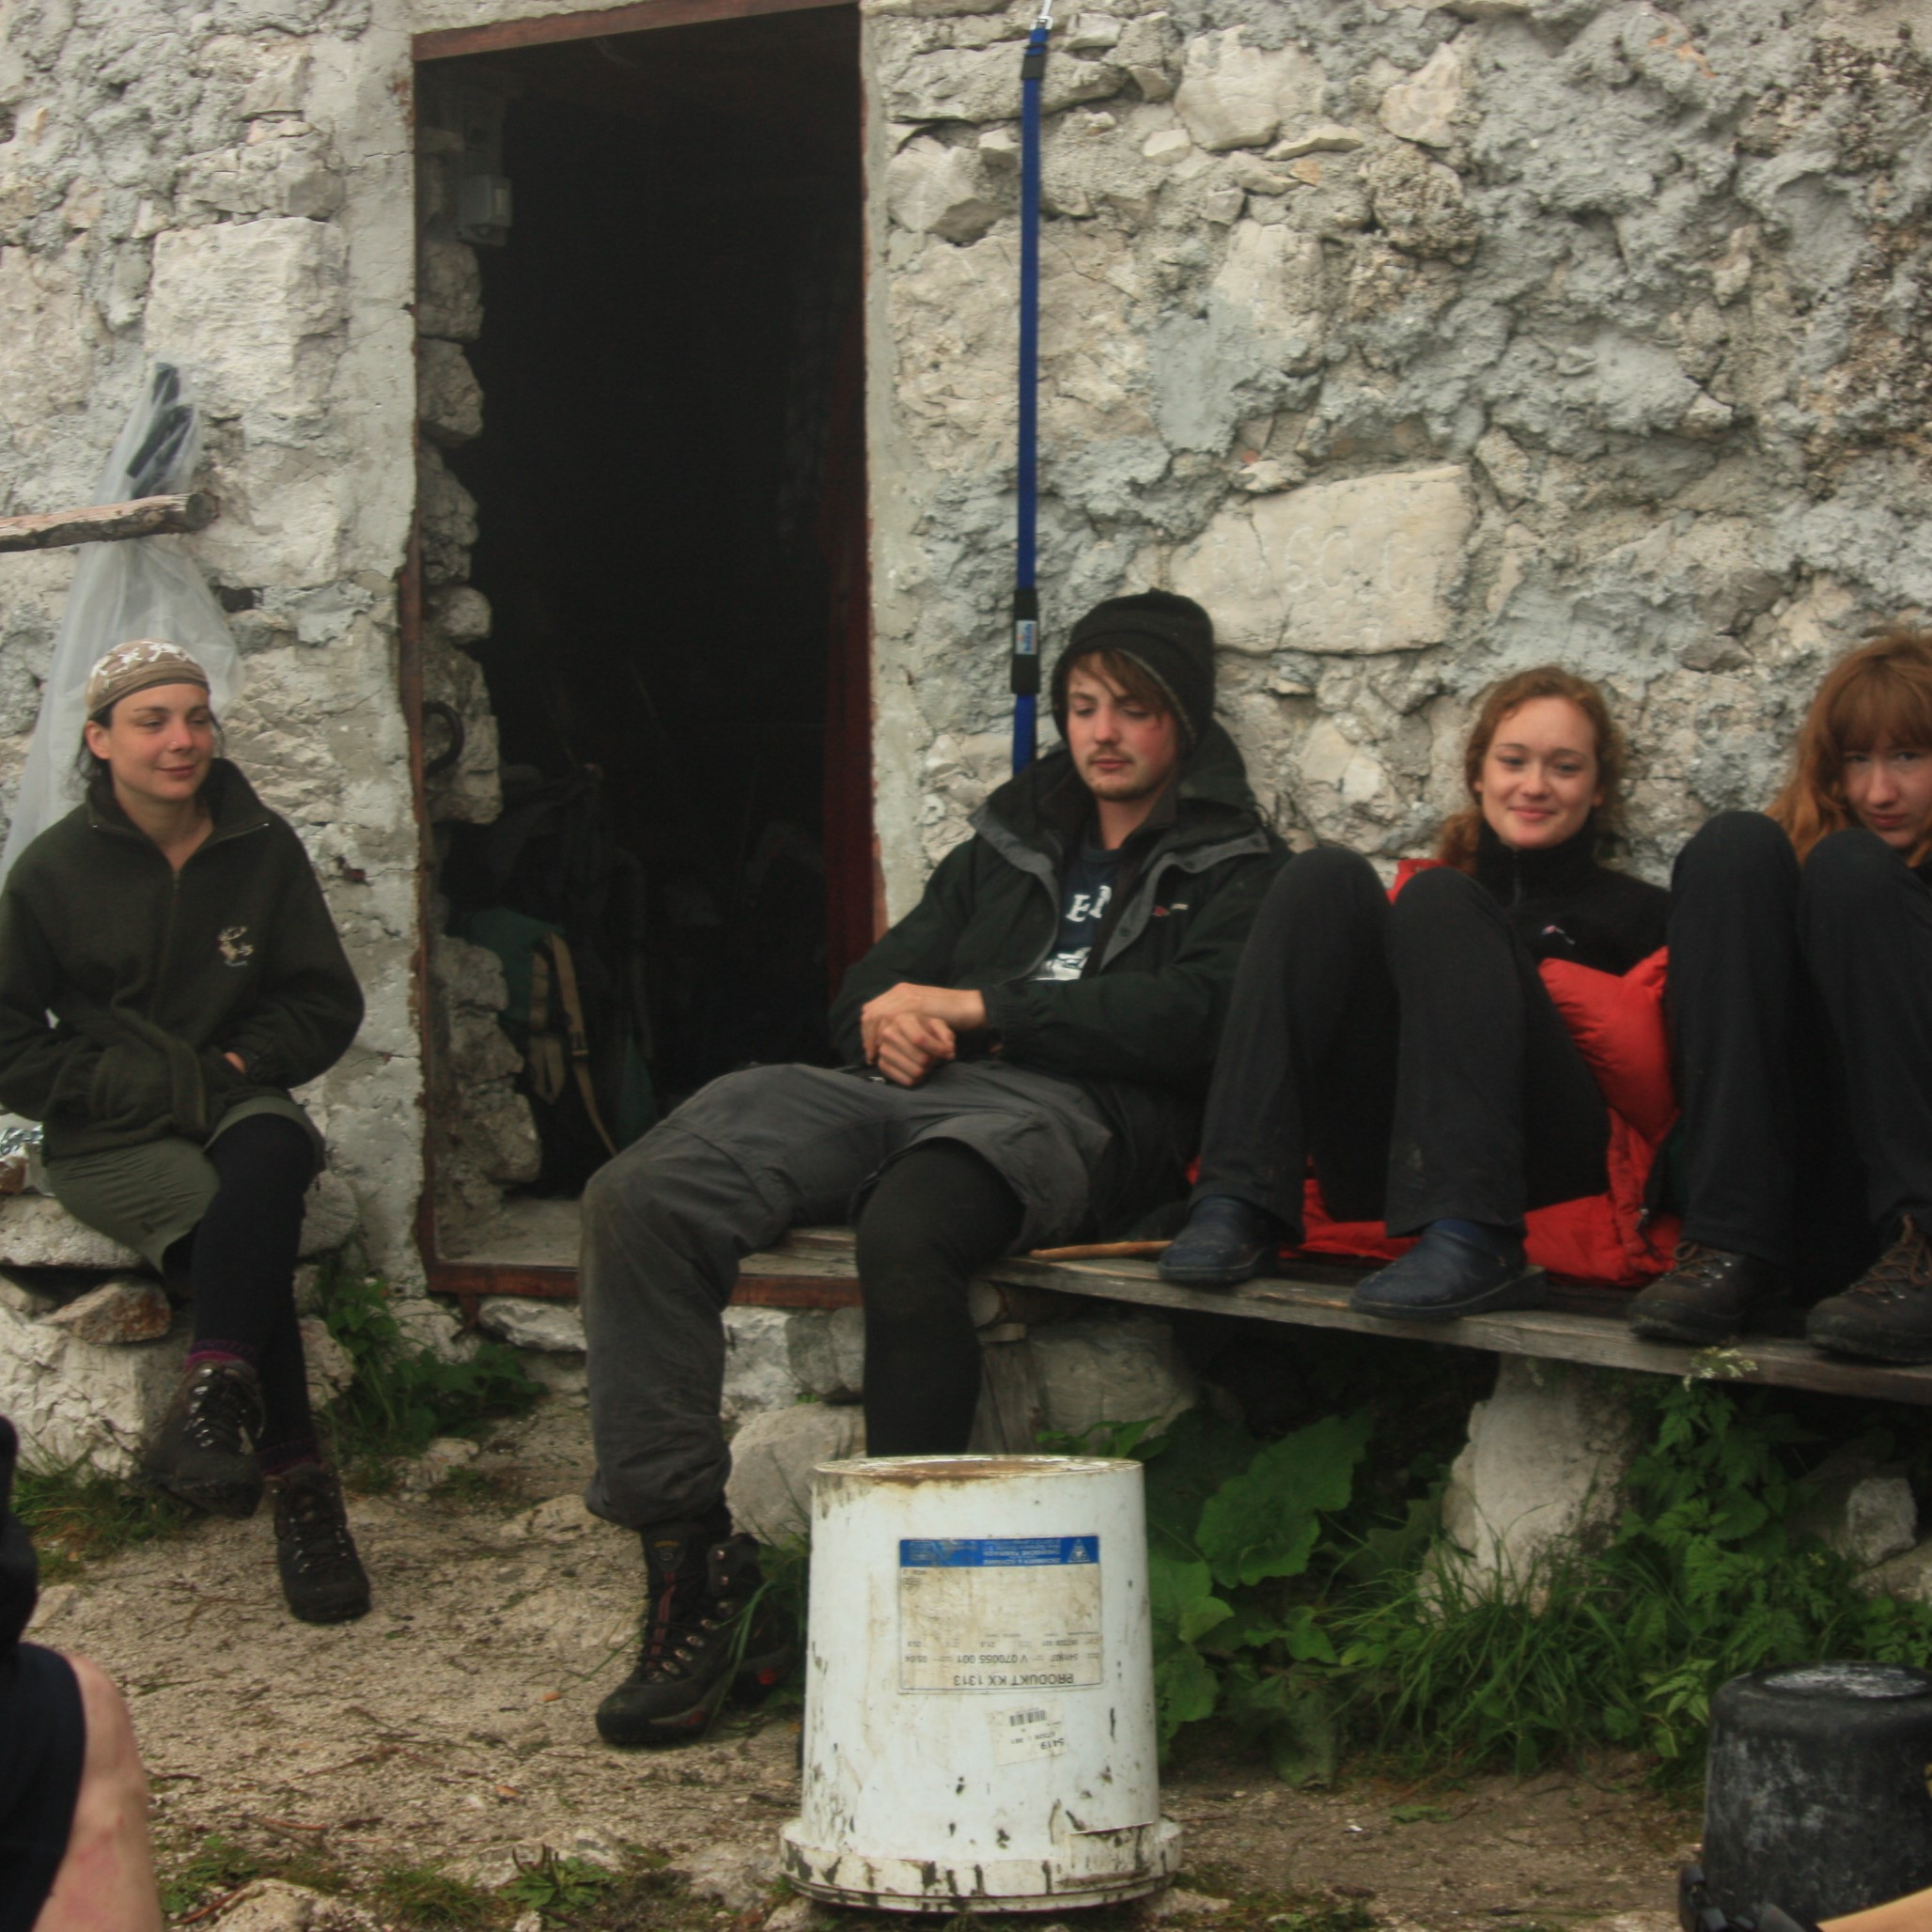
\includegraphics[width=\linewidth]{2011/alex_pitcher_award/zdenko/2011-08-07-09.09.51-Gergely Ambrus-Canon450D-IMG_1203-Zdenkos 50th Birthday Party at Kal--orig.jpg}} 
 \caption{On the morning after the night before, Jonny contemplates what happened to his missing trouser leg. \pic{Gergely Ambrus}}
 \label{jonny leg}
\end{marginfigure}

Once again, descending was enjoyable, the trip down now feeling familiar
and all the awkward pitches now being much more manageable. We arrived
at the top of \passage{Zimmer} in good time where myself and the person I
was caving with, Kate, were to collect a tackle bag each and head back
the way we came. Unfortunately, not all the bags were at \passage{Zimmer}
yet so I was elected to head to camp and carry a couple of tackle bags
back up \passage{Zimmer}. I made it down to camp to find a couple of
furious cavers who couldn't understand why I was sent down to camp when
I was a fresher. They also worked out that one of them would be carrying
two tackle bags the whole way out of the cave, something not many people
would envy.

\begin{pagefigure}
\checkoddpage \ifoddpage \forcerectofloat \else \forceversofloat \fi
   \centering
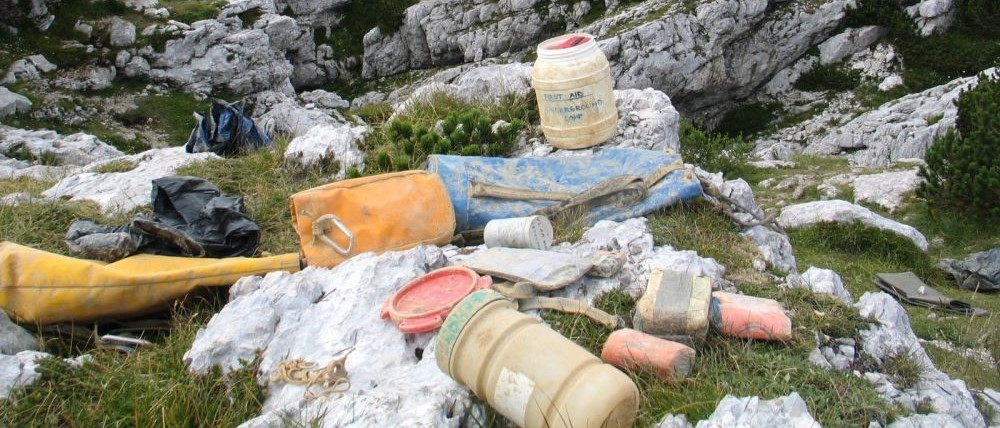
\includegraphics[width = \textwidth]{2011/alex_pitcher_award/2011-08-10-11.37.14-Jarvist Frost-CanonG5-IMG_0186 - Drying Underground Camp gear in the Sun--orig_1050p.jpg}
\caption{Ideally caving equipment will be dry for the journey down the mountain. Fortunately there was some sunshine to facilitate drying on the morning after the derig. \pic{Jarvist Frost}} \label{ug gear drying}
\end{pagefigure}

Nevertheless, we pressed on and I enjoyed my excursion down
to camp: it gave me a last chance to say farewell for the year. The
cave, however, seemed much wetter than usual and \passage{Zimmer},
especially the middle third, was really quite unpleasant. As such, I
felt quite cold upon making it to the top: it wasn't serious, just a
minor inconvenience. Myself and Kate began to head out the cave at a
steady pace. By the end of \passage{Pink}, Kate was beginning to feel quite
tired and I was beginning to feel cold.

A lot of the more experienced cavers find ways to keep themselves amused
whilst waiting for people to head up the rope. On my first couple of
trips with Tetley he took a book with him that he would read. Dave would
constantly be analysing the geology of the cave and looking out for
interesting pieces of cave (a hobby that led to him discovering
\passage{Kamikaze}, the most extensive lead of the year). To keep morale up,
\bignote{both of them would sing: Dave, quite sparingly, Tetley incessantly}. So,
in no way an experienced caver, I just sat in silence with my thoughts.
Ascending this time however, Kate asked me to sing to help boost morale.
I have no idea what she must have thought but all I know is that, to
begin with, I can't sing very well and secondly, the only songs I could
think of that day were excerpts from the \textit{Lion King} soundtrack. I was
glad when another caver, Clare, caught up with us and began singing
herself.



\begin{figure}
\checkoddpage \ifoddpage \forcerectofloat \else \forceversofloat \fi
   \centering
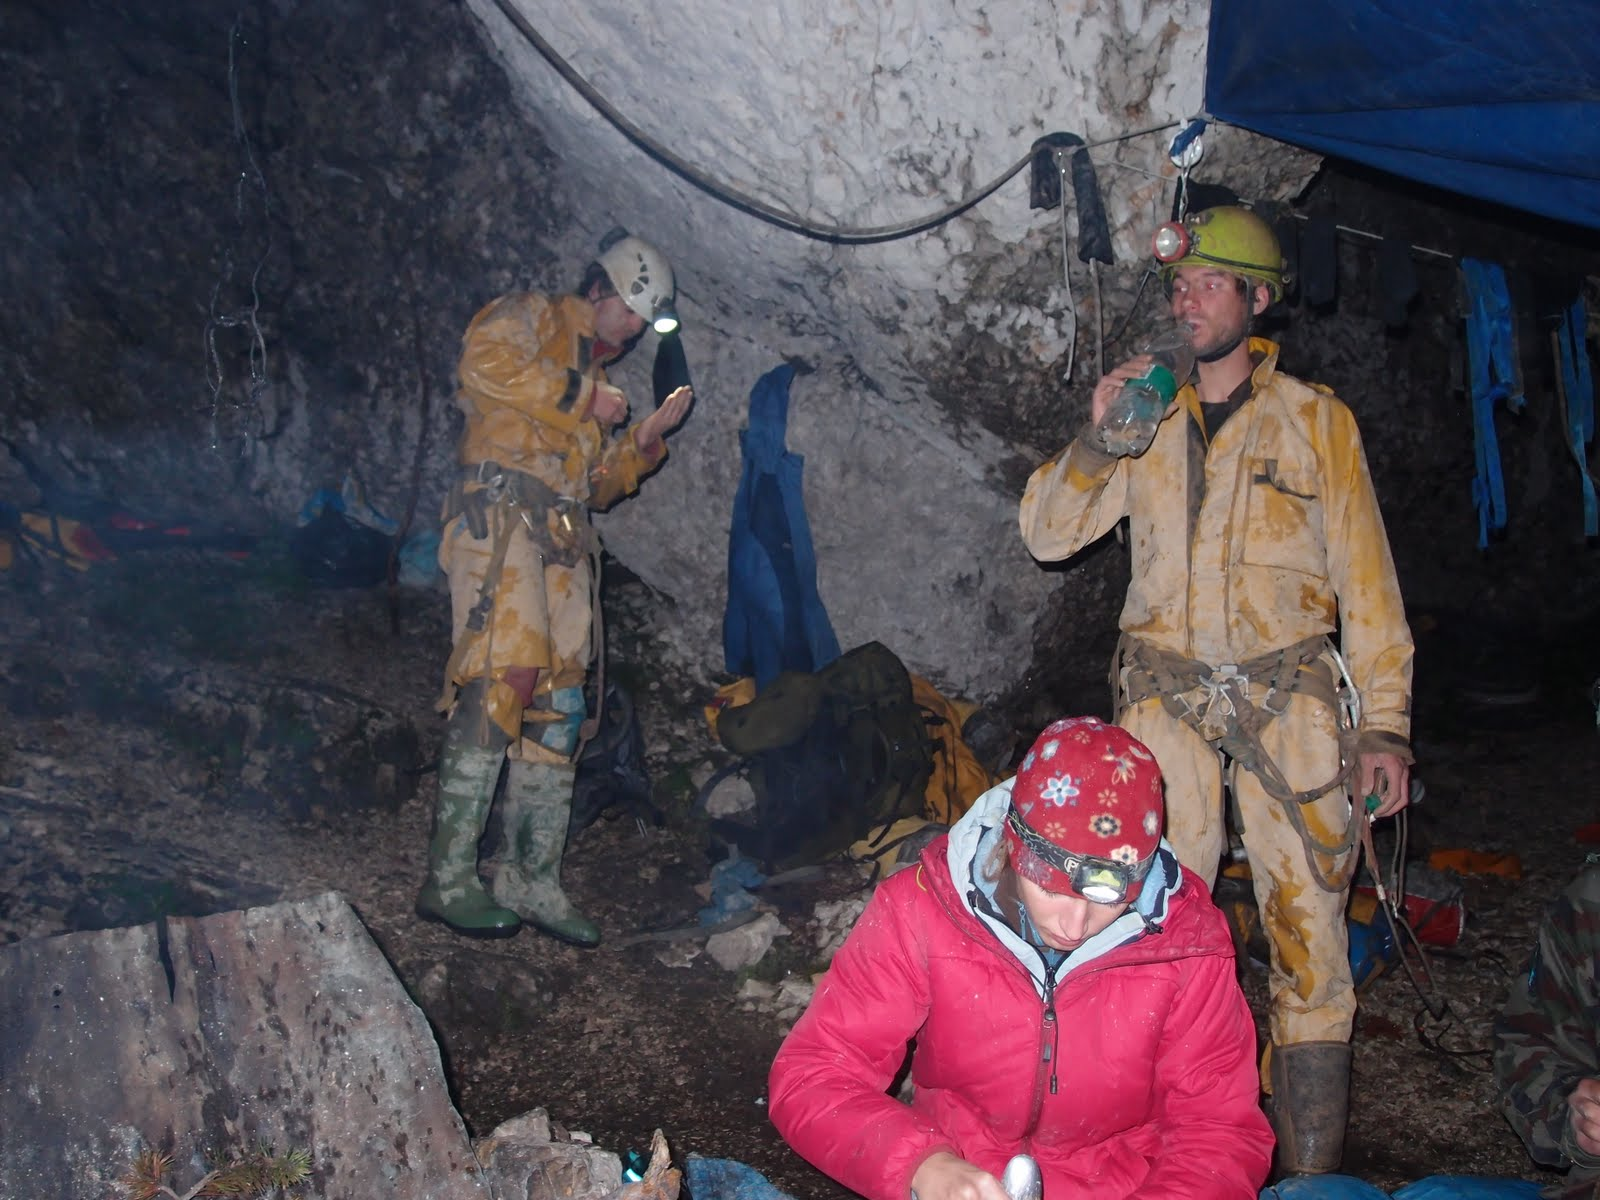
\includegraphics[width = \textwidth]{2011/alex_pitcher_award/2011-08-09-22.45.35-Andy Jurd-P8091892--orig.jpg}
\caption{Jonny and Gergely, still clad in caving gear, return to the bivi after their derig shifts. \pic{Andy Jurd}} \label{derig end}
\end{figure}

At this point I was beginning to feel quite cold and disheartened myself
so, to avoid becoming too uncomfortable and to also help avoid a
potential traffic jam, I began to follow a Hungarian named Gergely out
of the cave (as he sped along with two tackle sacks) and left Kate with
the dulcet tones of Clare shouting `You Are My Sunshine.'


\tweet{1:19PM Aug 10th, 2011}{Cave derig complete 5AM,another safe\&productive year to report.Sun and stunning viz for carries. Updates and surveys once down in valleys!}

We emerged to
a breezy rainy night at around 10 pm. The last caver out, Jarv, emerged
with the hangers and maillons at around 3 o'clock in the morning, a
herculean effort. And so, the last caving trip of Slovenia was over. We
spent the next day beginning the carries of equipment down the hill,
particularly caving gear. That night, we finished off the remainder of
the alcohol and stayed up late, enjoying our last night in the \passage{Bivi} next
to a roaring fire, accompanied by an excellent meal cooked by Gergely.



\subsection{End of expo}

The next day, the tents were packed up, the Bivi emptied and the rest of
the supplies packed messily in the mini van and taken to \passage[town]{Tolmin}.

Once again taking the bike down to \passage[town]{Tolmin}, this time with another ICCC
member, Alex we took a different route to \passage[town]{Tolmin}. This proved to be much
more spectacular providing us with an incredible view from a bridge
known as the Devil's Bridge that the JSPDT use for their SRT training.
It left me certain of the knowledge that they must have a head for
heights. Furthermore, we passed the cave that `apparently' was the
inspiration for Dante's Inferno. However, it was decided that we had
done enough caving for the trip and that lazing in the sun at \passage[town]{Tolmin} was
more desirable than exploring a muddy show cave.

A final party was held on the last night by the JSPDT and I think we
were all glad when we had a thoroughly relaxed night of wine and food.
After saying our goodbyes, the minibus departed \passage[town]{Tolmin} for the last
time, this time in the direction of the UK. It was with excitement and
sadness that I saw the White Cliffs of \passage[town]{Dover} appear before me, marking
the end of what had been one of the hardest and most rewarding
experiences of my life.

\name{Jonathon Hardman}

\begin{pagefigure}
\checkoddpage \ifoddpage \forcerectofloat \else \forceversofloat \fi
   \centering
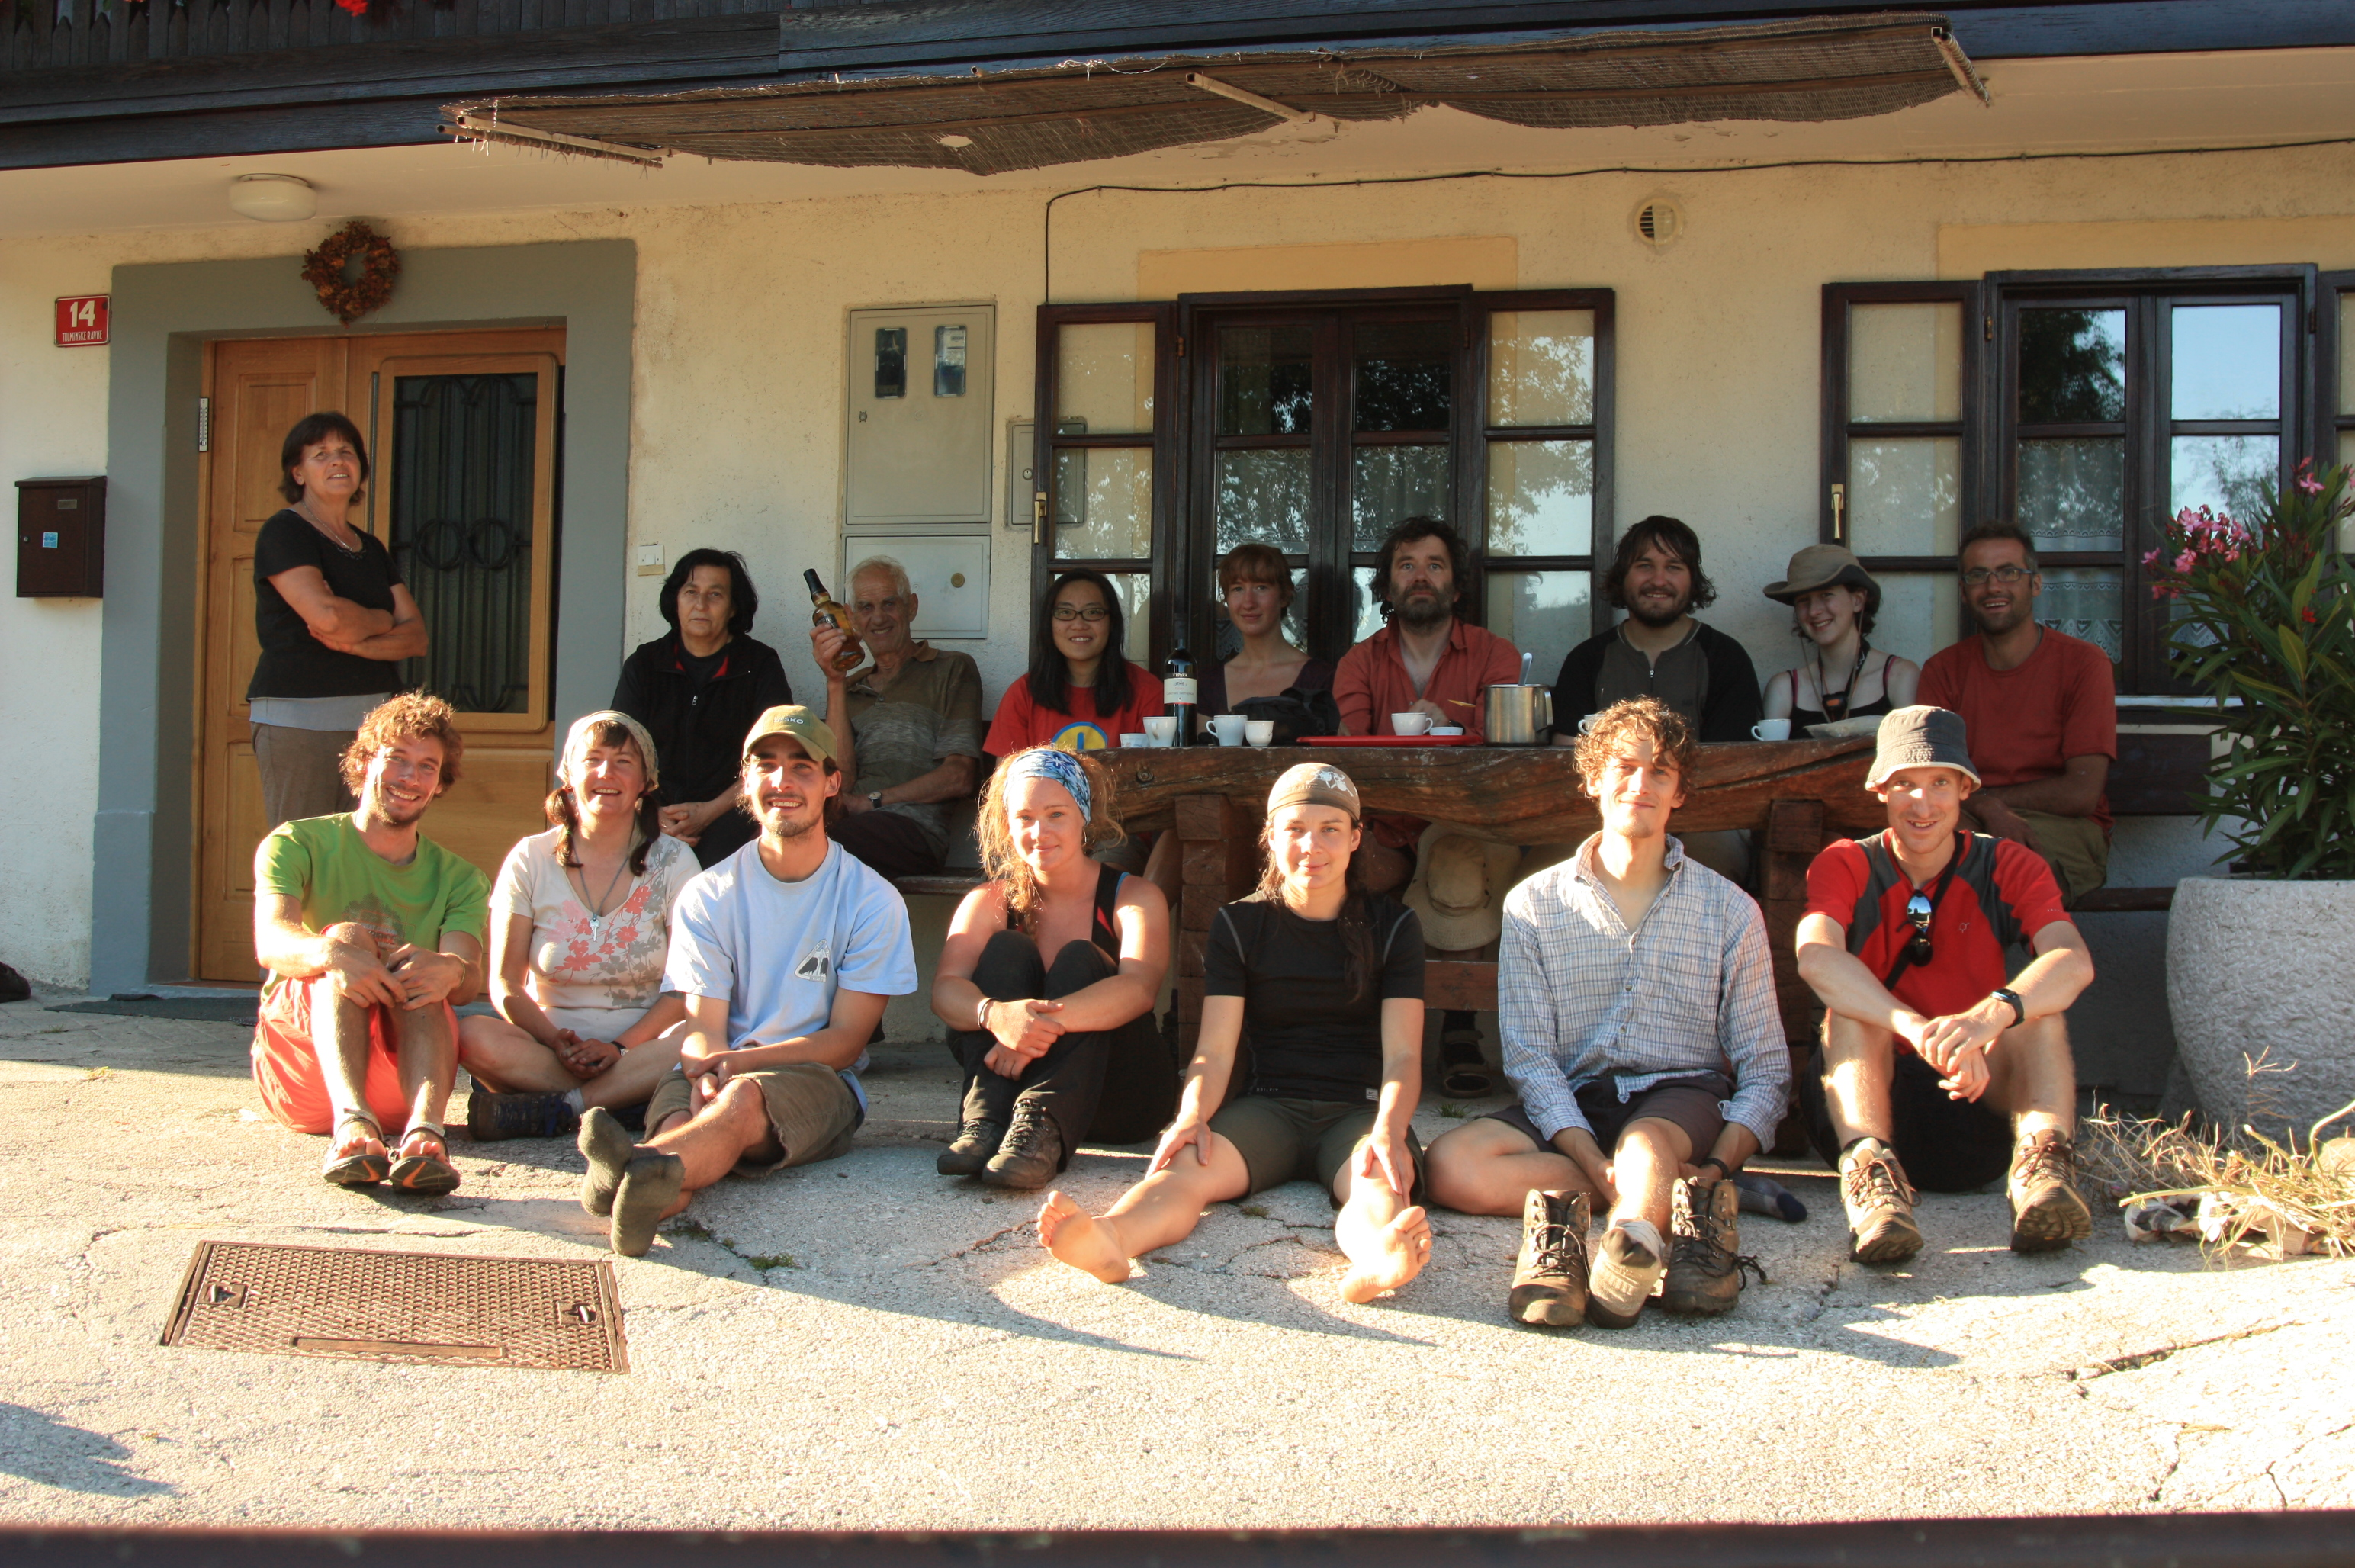
\includegraphics[width = \textwidth]{2011/alex_pitcher_award/2011-08-11-17.46.07-Gergely Ambrus-Canon450D-IMG_1396-Mountain Derig--orig.jpg}
\caption{\textit{left to right} Slavica Klobučar, Gergely Ambrus, Janet Cotter, ???, Izi Možir, Marjan Klobučar, Ari Whitby, Clare Tan, Kate Smith, Jana Čarga, Dave Wilson, Jarvist Frost, Alex Herriott, Nia John, Andy Jurd, Tetley. \pic{Gergely Ambrus.}} \label{Klobučar 2011}
\end{pagefigure}